\begin{figure}[htbp]
    \centering
    \begin{subfigure}[b]{0.48\textwidth}
        \includegraphics[width=\textwidth]{figures/Fig_Variance_Explained_30.png}
        \caption{30-dimensional latent space}
        \label{fig:variance_30d}
    \end{subfigure}
    \hfill
    \begin{subfigure}[b]{0.48\textwidth}
        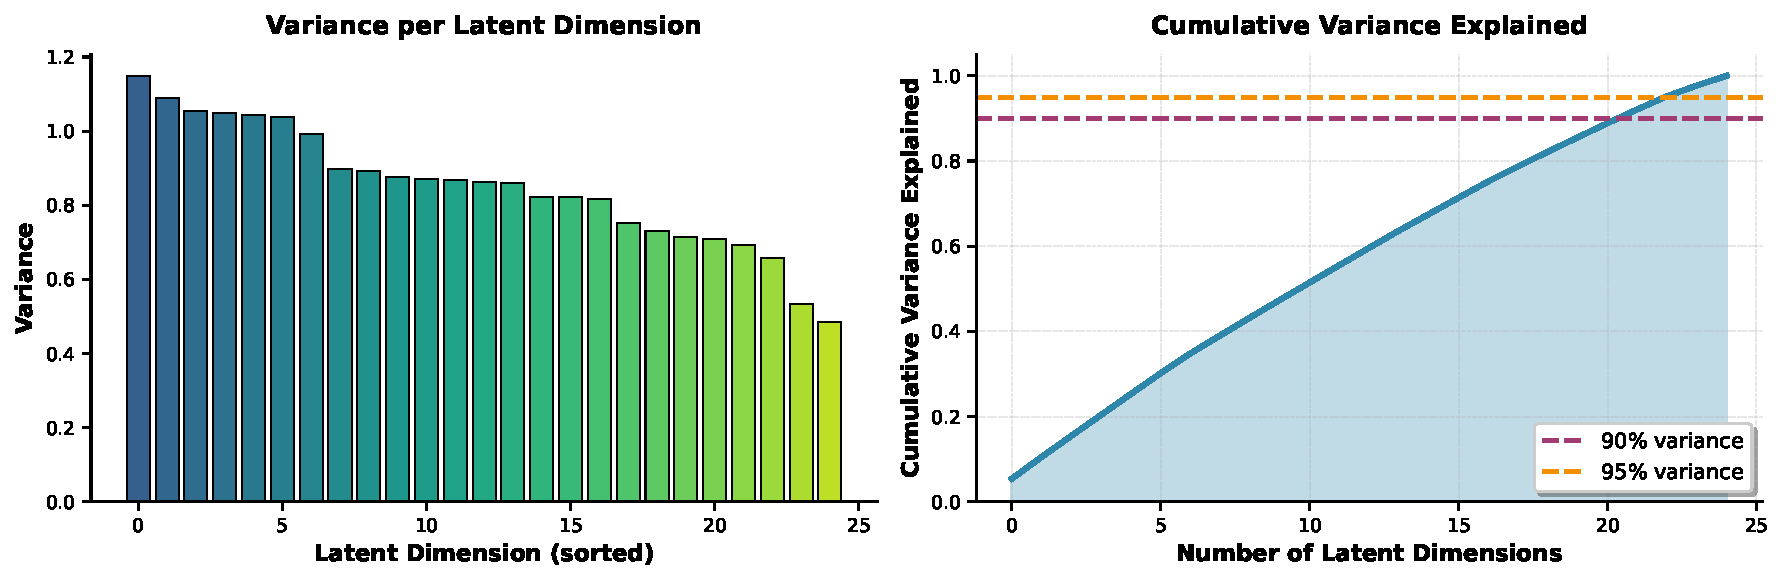
\includegraphics[width=\textwidth]{figures/Fig_Variance_Explained.png}
        \caption{50-dimensional latent space}
        \label{fig:variance_50d}
    \end{subfigure}
    \caption{\textbf{Variance distribution across learned latent dimensions.}
    Analysis of the LSTM-VAE's latent space reveals hierarchical information encoding across dimensions.
    \textbf{Left:} Individual variance per latent dimension (sorted in descending order) demonstrates uneven information allocation, with the first few dimensions capturing disproportionately large variance. This non-uniform distribution indicates structured encoding of dynamical features rather than diffuse, redundant representations.
    \textbf{Right:} Cumulative variance explained shows that $\sim$20--25 dimensions capture 90\% of total variance (purple dashed line), while 95\% (orange dashed line) requires most available dimensions.
    The smooth, monotonic accumulation without abrupt plateaus suggests continuous hierarchical encoding of dynamical complexity.
    Comparison between \textbf{(a)} 30-dimensional and \textbf{(b)} 50-dimensional configurations demonstrates that the 30-dimensional latent space achieves efficient compression with minimal information loss, justifying its selection for the final model architecture.
    The similar variance profiles between both dimensionalities indicate that 30 dimensions suffice to capture the intrinsic complexity of GLV dynamics in our dataset.}
    \label{fig:variance_explained}
\end{figure}
